\documentclass[a4paper]{article}

\usepackage[english]{babel}
\usepackage[utf8]{inputenc}
\usepackage{amsmath}
\usepackage{graphicx}
\usepackage[colorinlistoftodos]{todonotes}

\title{Electric Circuits 307 - Diodes}

\author{Josh Lofy}

\date{\today}

\begin{document}
\maketitle

\begin{abstract}
In this lab I will discuss how diodes, from LEDs to silicon and germanium diodes, function and how we can use them effectively to modify signals.  The circuits that will be discussed will be based on the ideas of clipping, rectifying (both half and full wave), and changing a AC signal to a DC signal using either a transformer or a bridge circuit.
\end{abstract}

\section{Introduction}

Our diodes in this lab worked as expected with little error.  We were able to map out the IV characteristics of the silicon diode through a theoretical calculation using Multisim v10.1.  This showed when current was flowing that the turn on voltage was around 540mV.  I will talk more about what this means, as well as how diodes are effectively modeled in a circuit.

Also, I will talk about the effectiveness of diodes as clipping circuits.  A clipping circuit does what it sounds like it does, it clips the input signal at a certain set voltage.  In our circuit this voltage was easily controlled by changing an outside DC source.

We also constructed two different kinds of rectifying circuits.  One circuit was a full wave rectifier, and the other was a half wave rectifier.  A full wave rectifier is the equivalent of taking the absolute value of the incoming AC signal if it is centered at V=0.  The half wave rectifier completely eliminated the negative value of our AC signal centered at the origin.  This can also be a kind of clipping circuit, with the exception being we have no way to control the amount of clipping for the negative portion of signal.

To easily see these changes we did use LEDs to see our signal traveling through the circuit.  However, this was only helpful for lower frequencies, and was coolest in the bridge circuit where we were able to create an array of green and red "Christmas" style lighting.

\section{The Circuits and Their Design}

\subsection{Materials Needed}

\begin{itemize}
\item Frequency generator 
\item DC voltage supply
\item Oscilloscope
\item Assorted wires
\item LED (Any color, but variety is helpful and more fun)
\item Silicon diode (1N914)
\item Germanium diode (1N34)
\item Breadboard
\end{itemize}

\subsection{IV Characteristics}

The IV characteristics of our diode can be described also as the area where our input signal is greater than the turn on voltage and our diode begins allowing current to flow through it.  Shown is Figure 1 is a diagram of how diodes are effectively modeled, with one arrow representing input signal and the other representing what happens to the output signal.

For our silicon diode (1N394), the turn on voltage was 540mV.

\begin{figure}
\centering
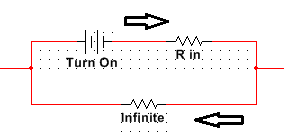
\includegraphics[width=.5\textwidth]{Diode_model.png}
\caption{\label{fig:Diode}Here is an effective model of a diode in a circuit}
\end{figure}

\subsection{Clipping Circuit}

In a clipping circuit we effective cut the voltage of the circuit at a certain point.  With the \todo{Example: Very high frequencies create angled cuts more resembling of triangle waves} exception of some situations, this slice is taken horizantally with respect to the origin.  The design is shown in Figure 2.

\begin{figure}
\centering
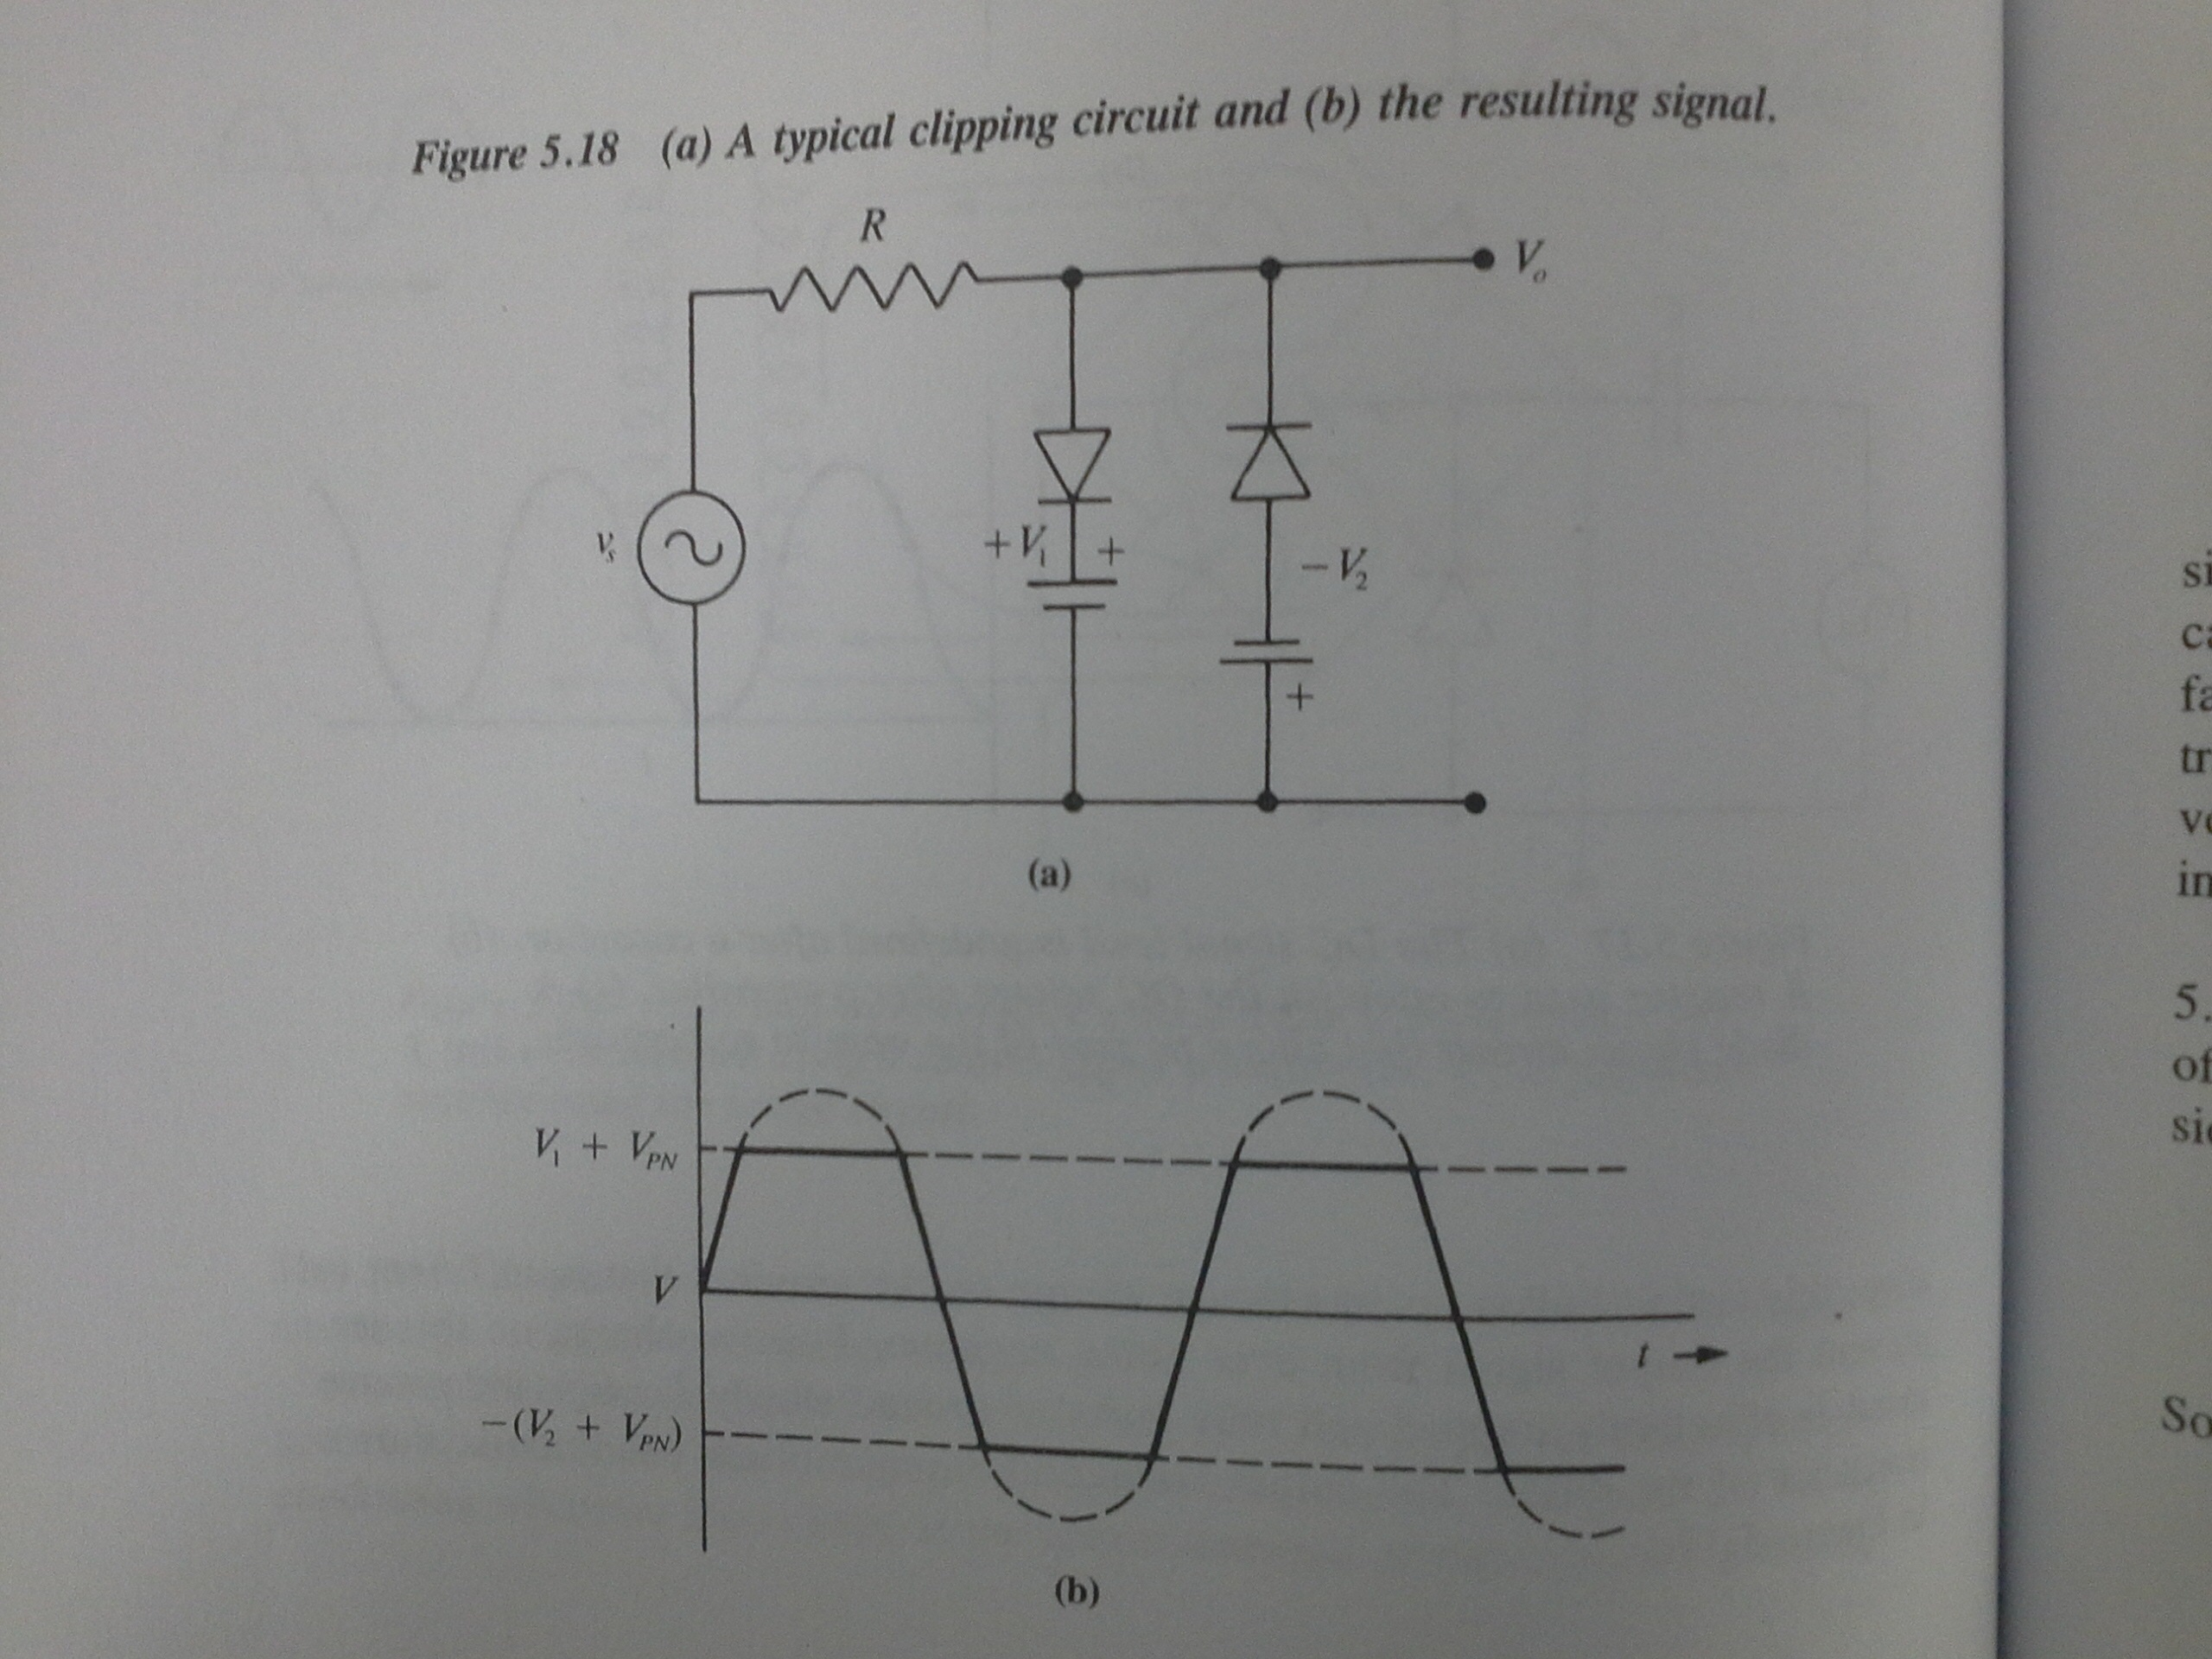
\includegraphics[width=.7\textwidth]{Clipping_Circuit_307book.jpg}
\caption{\label{fig:Clipping}This is a photo from our textbook, Principles of Electronics, showing a design for a clipping circuit and it's theoretical output}
\end{figure}

Where the DC power sources are on the Figure are where we placed our DC power sources.  We were then able to use the dials on the DC power source to change the amount that the diode cut off.

\subsection{Half Wave Rectifier}

A half wave rectifier was easily constructed using one diode and a load resistor to measure the signal across.  The signal for this rectifier looks like only the top halves of the sine wave input signal. \todo{An exception to this would be if the signal were extremely large} This circuit shows us that the diodes will only allow through the signal in one direction.

\subsection{Full Wave Rectifier}

The full wave rectifier is used to make all of our signal flip across the origin.  This is the same as if we were to take the absolute value of the input signal, assuming our origin is at V=0.  The full wave rectifier was designed as two different circuits.  One of the circuits used a transformer.  For our transformer circuit, we set it up as shown in Figure 3.  

\begin{figure}
\centering
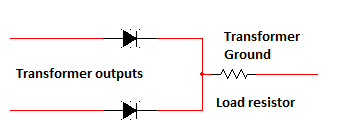
\includegraphics[width=.5\textwidth]{AC_to_DC_figure.png}
\caption{\label{fig:ACDC}Here is our circuit set up without the transformer in picture.  The transformer has 3 wires.  2 of the wires supply an input signal, while the third acts as a ground.}
\end{figure}

The second part of our Full wave rectifier circuit involves using the frequency generator and a bridge circuit.  The Bridge circuit that we designed used the LEDs.  This was one of our most fun circuits as this is where we set up a series of blinking lights that went back and forth, showing us \todo{LEDs were only effective like this with low enough frequencies for our eyes to see} exactly how the signal traveled through the diodes.  The bridge circuit is shown in Figure 4.

\begin{figure}
\centering
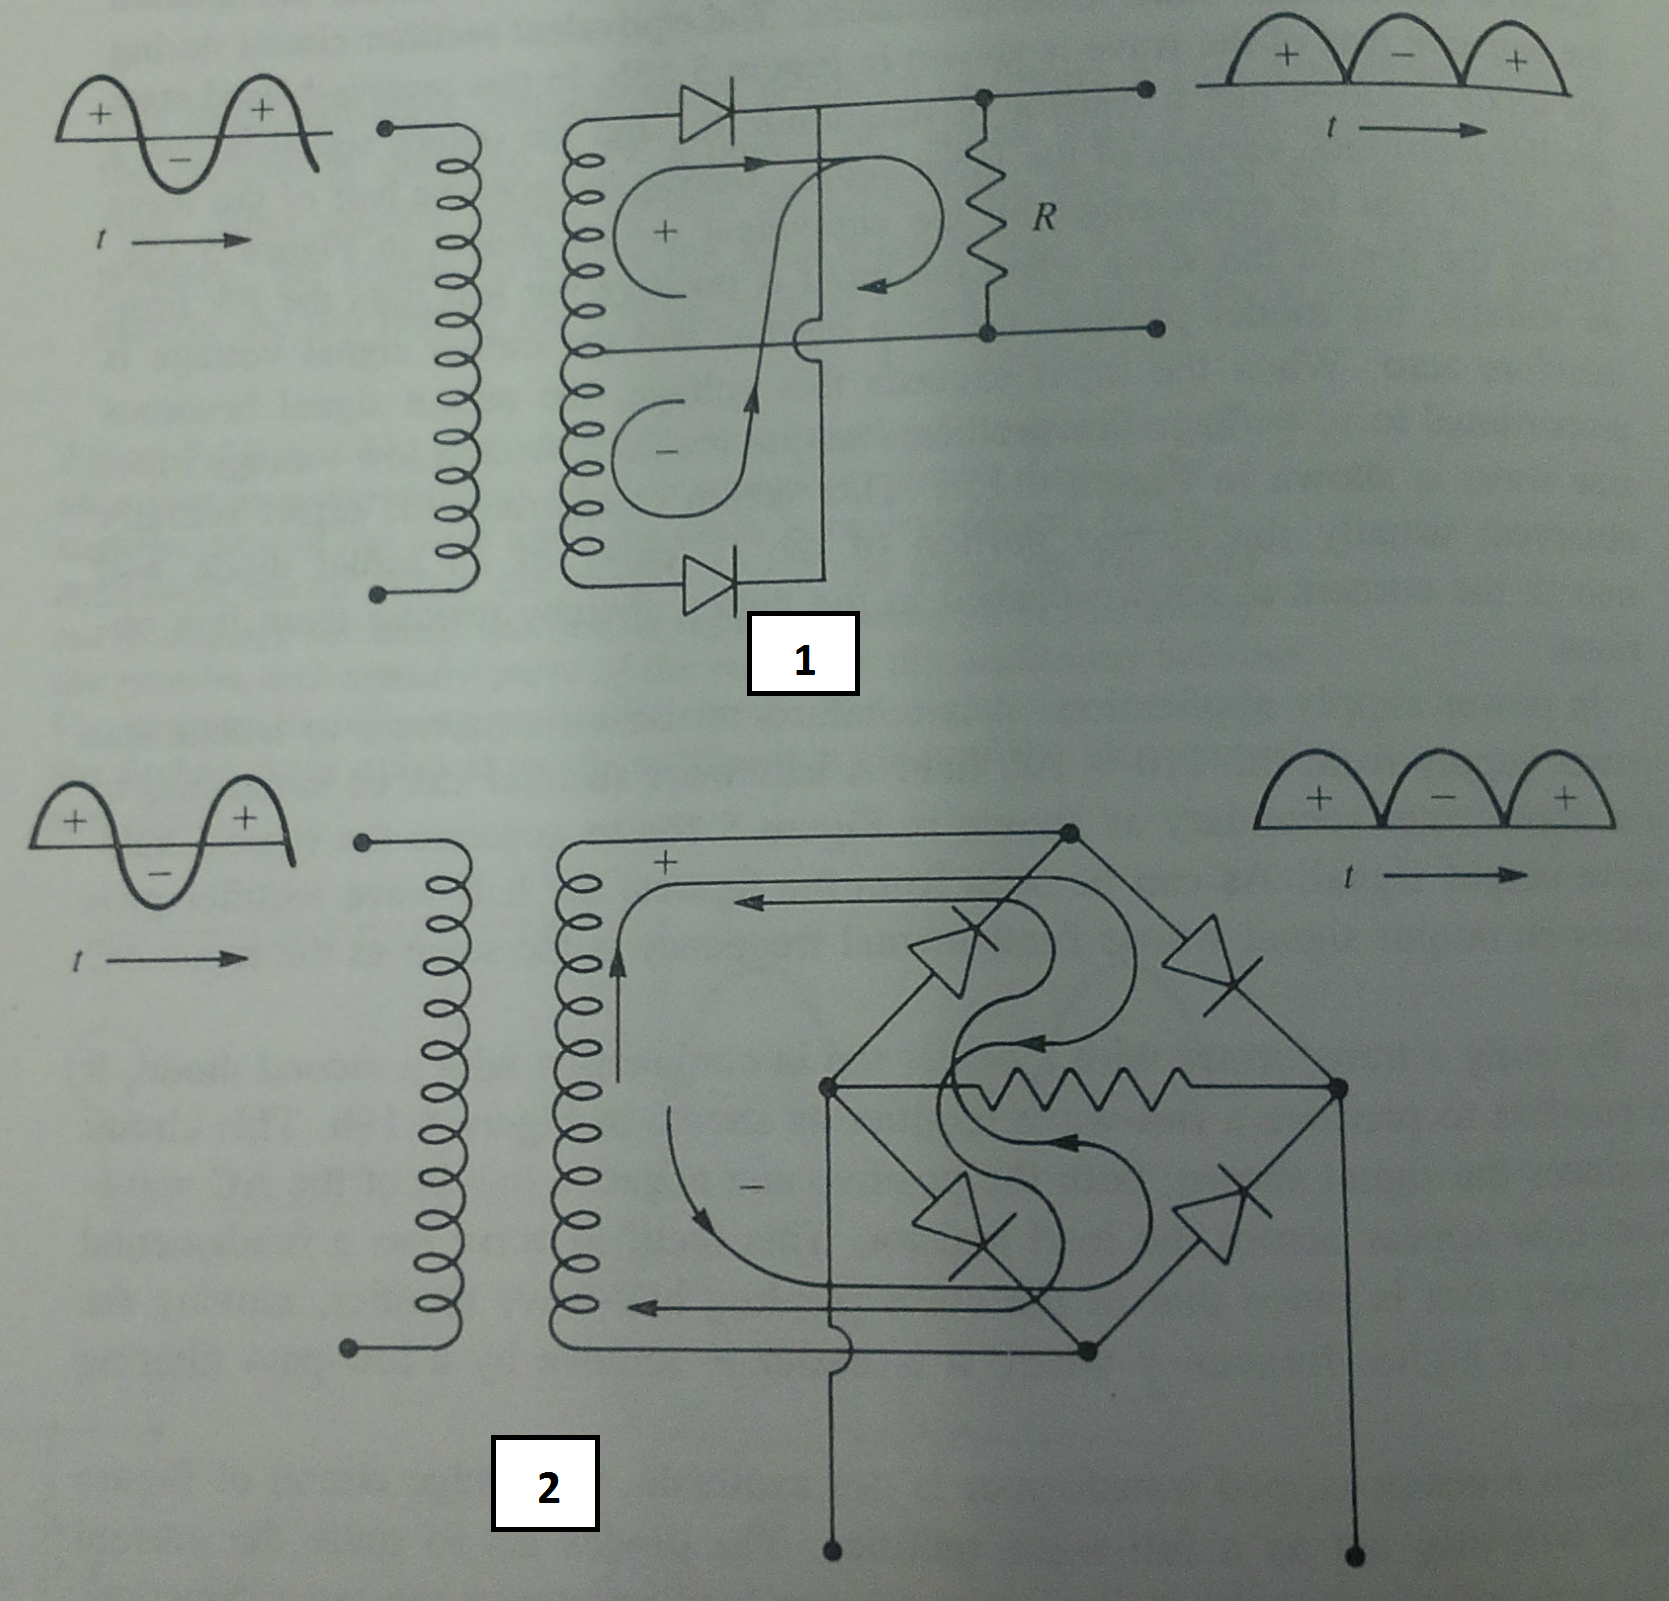
\includegraphics[width=.65\textwidth]{Rectifier_circuits.png}
\caption{\label{fig:Rect} 1)A transformer full wave rectifier circuit 2)A bridge circuit.  Both are useful for creating AC to DC signals.  Photo taken from our textbook, Principles of Electronics.}
\end{figure}

\begin{figure}
\centering
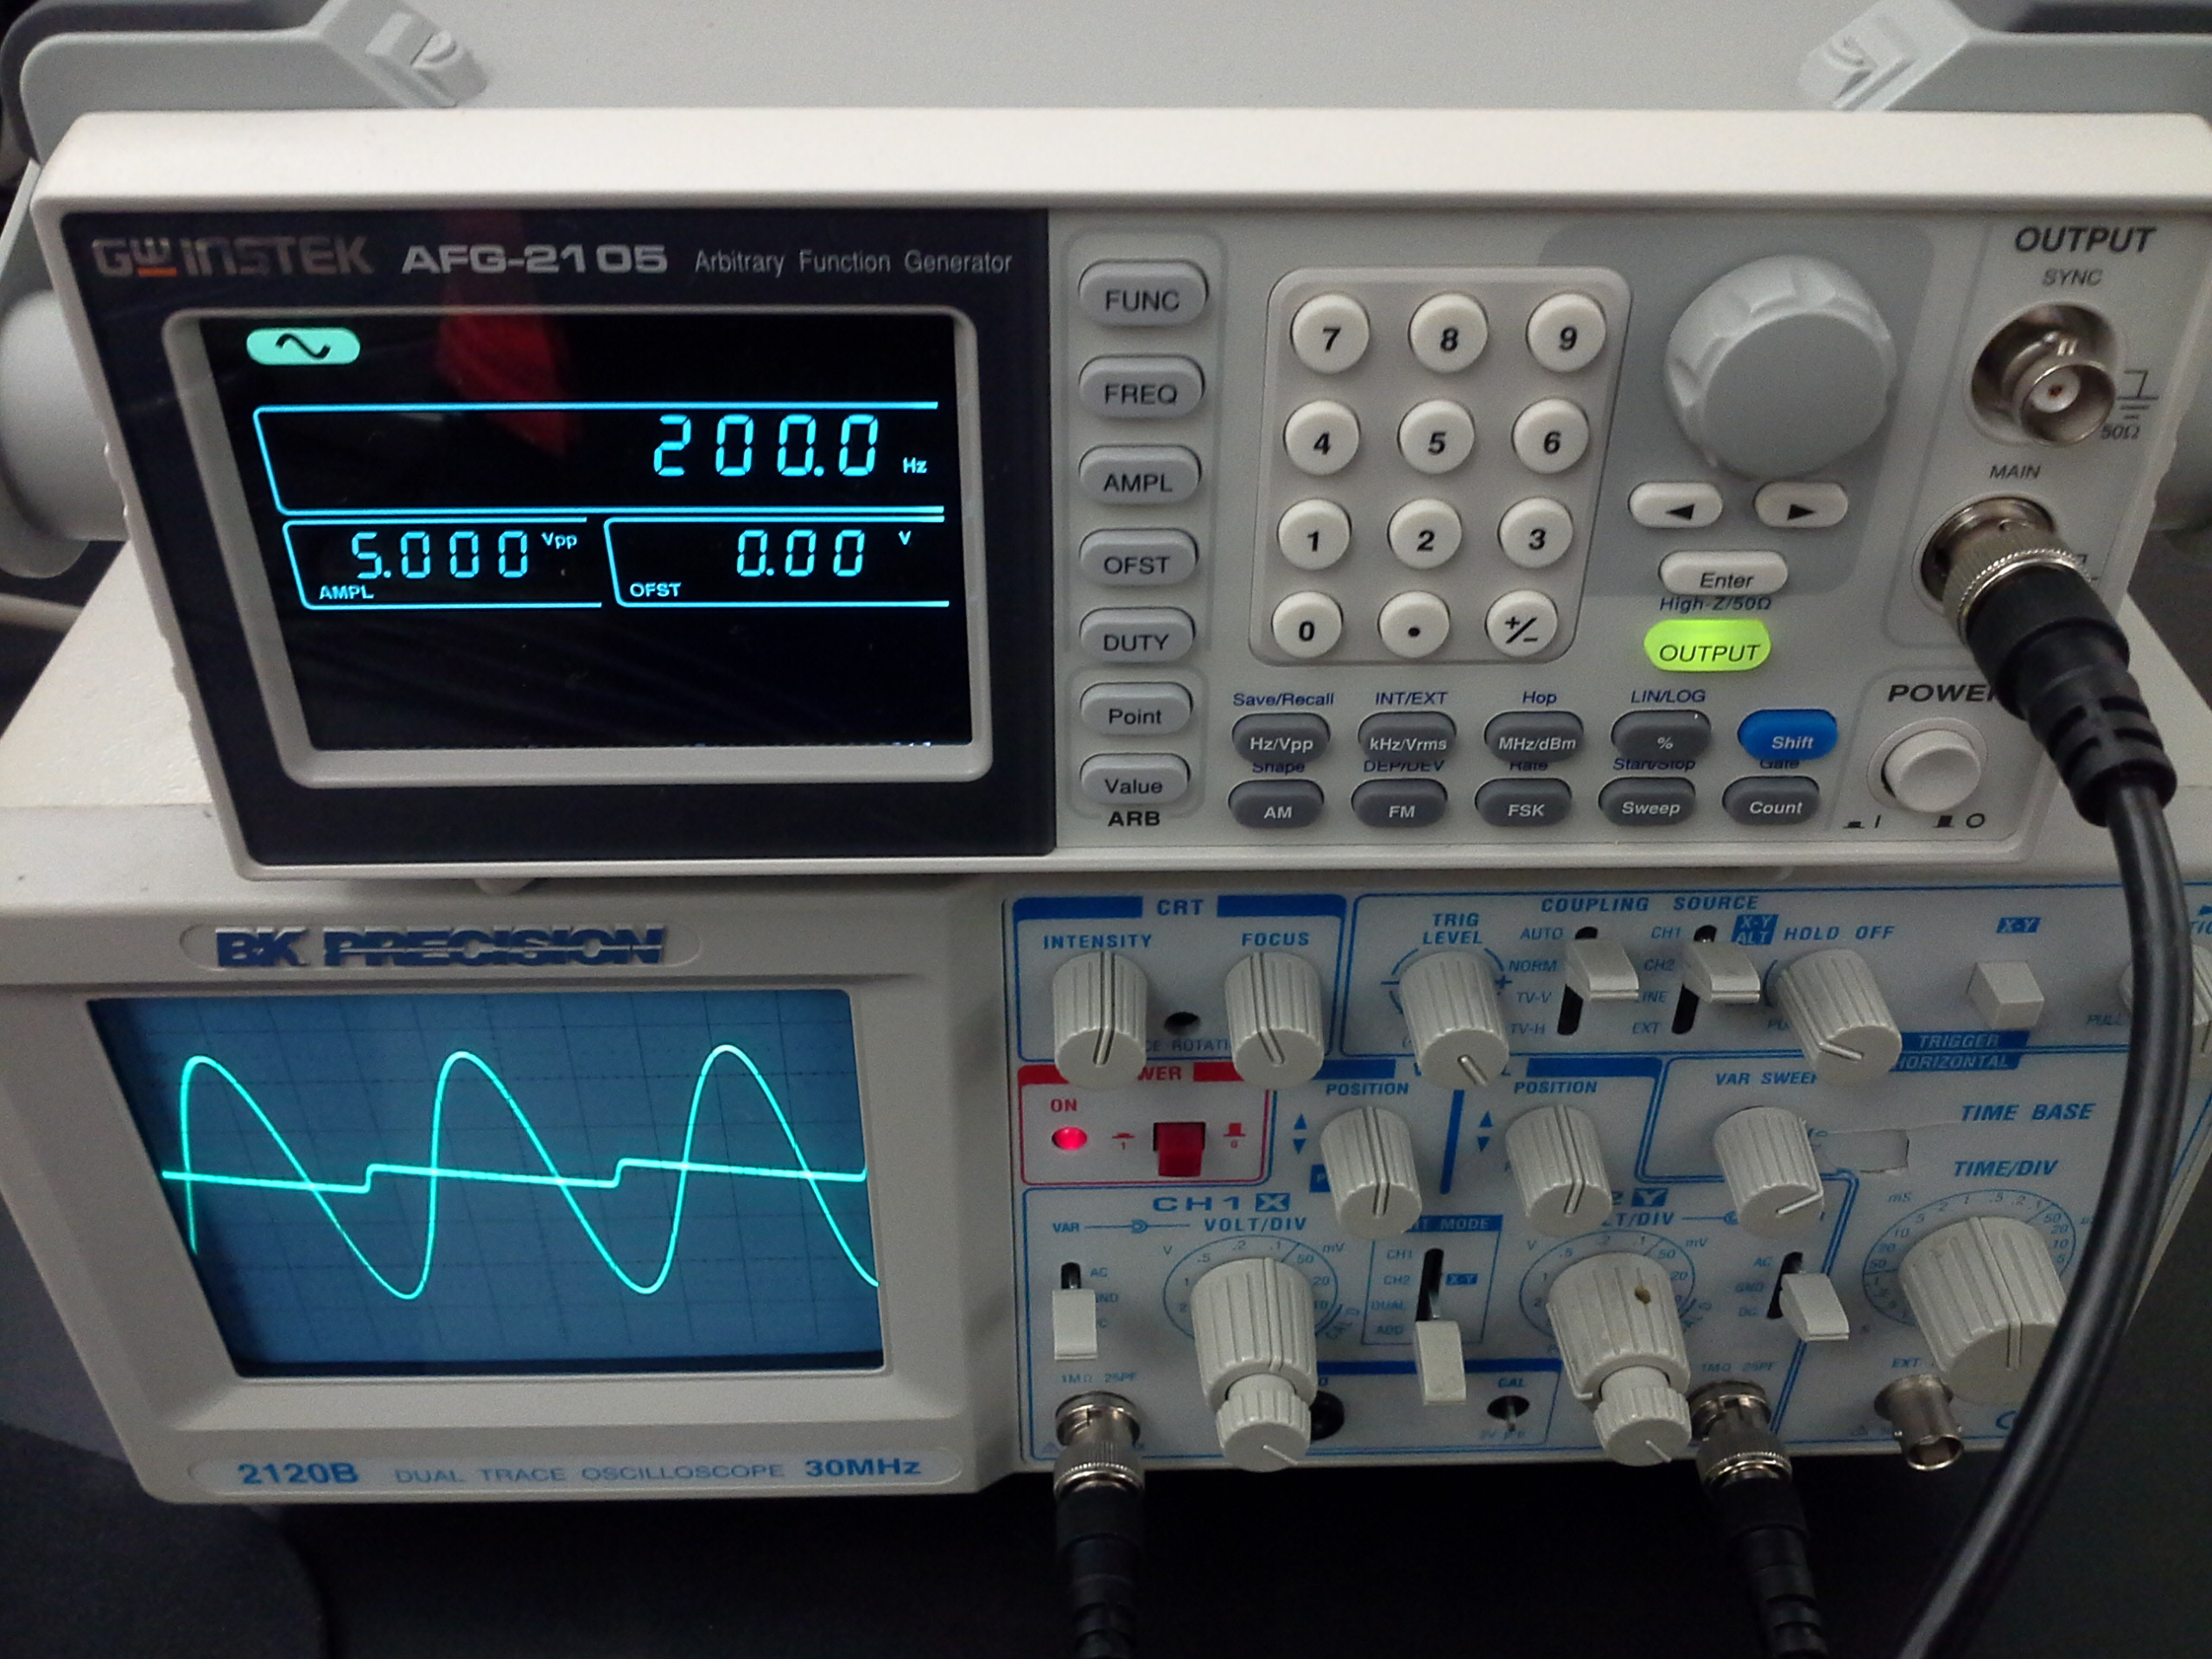
\includegraphics[width=.5\textwidth]{ACDC.jpg}
\caption{\label{fig:RectMeasured}Our measurement of our AC to DC circuit}
\end{figure}

\section{Conculsion}

We were able to set up all of the assigned circuits in a variety of different ways, both with and without the frequency generator and transformer.  These circuits have many uses when applied to signals, and are important for signal control and understanding of how to create a better DC signal from an AC outlet.  

\end{document}